A curb extension (\figref{curb-extension}) is an extension of the curb onto the roadway. As a traffic calming measure, they are primarily used to assist pedestrians by reducing crossing distance and slowing traffic down.

\begin{figure}[h]
\centering
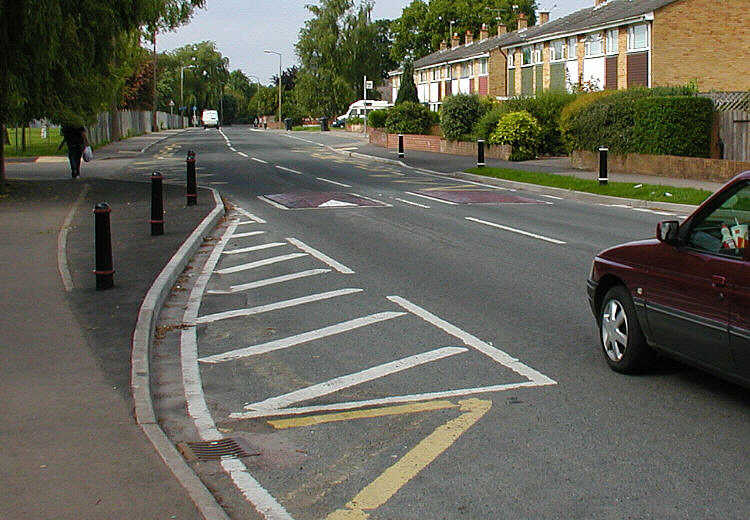
\includegraphics[width= 0.5\textwidth]{curb-extension}
\caption{Curb extension}\label{fig:curb-extension}
\end{figure}

\subsubsection{Advantages and Disadvantages}

Curb extensions are thought to have the following advantages:\begin{itemize}
\item Reduce the time that pedestrians are exposed to traffic.
\item Increase the visibility of pedestrians attempting to cross.
\item Shield parking lanes from oncoming traffic and prevent drivers from using them as right turn lanes.
\end{itemize}

The various drawbacks are:\begin{itemize}
\item They pose a threat to bicyclists, who are forced into a narrowed gap along with traffic.
\item Like raised crosswalks, they complicate drainage since they obstruct the gutter.
\item Reduce the availibility of parking spaces, which can hurt local businesses.
\end{itemize}

\subsubsection{Effectiveness}

One study \cite{randal05} found that curb extensions significantly reduced the number of vehicles pedestrians had to wait for before one yielded. The same study also found minor increases in percents of crossings where a motorist yielded, and of vehicles yielding at advance stop bars. These results are shown in Tables ~\ref{table:vehicles-passed}, \ref{table:motorist-yielded} and \ref{table:motorist-stop-bar}.

% Booktabs require to add \usepackage{booktabs} to your document preamble
\begin{table}[!htbp]
\centering
\begin{tabular}{@{}crrrr@{}}
\toprule
\multicolumn{1}{l}{Lane} & \multicolumn{1}{l}{Non-curb extension} & \multicolumn{1}{l}{Curb extension} & \multicolumn{1}{l}{Difference} & \multicolumn{1}{l}{Sample Size} \\ \midrule
Near                     & 2.58                                   & 1.81                               & -42.7 \%                            & 219                             \\
Far                      & 2.36                                   & 1.76                               & -33.9  \%                           & 214                           \\
\bottomrule 
\end{tabular}
\caption{Average number of vehicles passing before a pedestrian-cross. Results found significant by the t-test.}\label{table:vehicles-passed}
\end{table}
% Booktabs require to add \usepackage{booktabs} to your document preamble
\begin{table}[!htbp]
\centering
\begin{tabular}{@{}crrrr@{}}
\toprule
\multicolumn{1}{l}{Lane} & \multicolumn{1}{l}{Non-curb extension} & \multicolumn{1}{l}{Curb extension} & \multicolumn{1}{l}{\% difference} & \multicolumn{1}{l}{Sample Size} \\ \midrule
Near                     & 64.9\%                                 & 66.7\%                             & 2.7\%                             & 234                             \\
Far                      & 58.6\%                                 & 63.4\%                             & 7.7\%                             & 234                            \\
\bottomrule
\end{tabular}
\caption{Percents of pedestrian crossings with yield. The results were found insignificant by the t-test.}\label{table:motorist-yielded}
\end{table}
% Booktabs require to add \usepackage{booktabs} to your document preamble
\begin{table}[!htbp]
\centering
\begin{tabular}{@{}crrrr@{}}
\toprule
\multicolumn{1}{l}{Lane} & \multicolumn{1}{l}{Non-curb extension} & \multicolumn{1}{l}{Curb extension} & \multicolumn{1}{l}{\% difference} & \multicolumn{1}{l}{Sample Size} \\ \midrule
Near                     & 42.6\%                                 & 53.8\%                             & 21.0\%                            & 99                              \\
Far                      & 42.6\%                                 & 51.9\%                             & 18.0\%                            & 99                            \\
\bottomrule 
\end{tabular}
\caption{Percent of vehicles yielding at advance stop bar. The results were found insignificant by the t-test.}\label{table:motorist-stop-bar}
\end{table}

\subsubsection{Cost and Considerations}

Curb extensions cost between \$5,000 and \$25,000 per corner\cite{walking-info-enhancements}. As with most sidewalk retrofitting, a large portion of the cost goes to drainage. If it is also necessary to remove a utility pole or other such existing infrastructure element, costs can become much higher.